\documentclass[11pt]{article}

\usepackage[margin=1in]{geometry}
\usepackage{amsmath,amssymb}
\usepackage{booktabs}
\usepackage{graphicx}
\usepackage{caption}
\usepackage{hyperref}
\setlength{\emergencystretch}{3em}

\hypersetup{
  colorlinks=true,
  linkcolor=blue,
  citecolor=blue,
  urlcolor=blue
}

\title{Comparative Evaluation of Multi-Omics Learning Models\\for Cancer Prediction with Breast Cancer External Validation\\and a Multi-Cancer Internal Benchmark}
\author{
Zhequan Hu\textsuperscript{1},
Xingang Bi\textsuperscript{1,*}\\
\textsuperscript{1}Department of Urology, National Cancer Center, Beijing, China\\
Cancer Hospital, Chinese Academy of Medical Sciences\\
and Peking Union Medical College, Beijing, China\\
\textsuperscript{*}Corresponding author: Professor Xingang Bi, bixingang@csco.org.cn
}
\date{\today}

\begin{document}
\maketitle

\begin{abstract}
Liquid neural networks have been proposed as continuous-time recurrent models that can adapt hidden-state dynamics to input-dependent rates. Their suitability for cross-sectional cancer multi-omics prediction remains unclear because most multi-omics cohorts are not natural temporal sequences. We evaluated a closed-form Liquid/CfC-style model for breast cancer molecular subtype prediction using TCGA-BRCA and METABRIC as a joined training pool, followed by independent external validation on CPTAC 2020, SMC 2018, and GSE96058/SCAN-B. To address the limitation of a single-cancer benchmark, we further constructed a five-task TCGA PanCancer internal benchmark covering UCEC molecular subtype, COADREAD molecular subtype, HNSC HPV status, KIRC grade, and PRAD pathologic T stage. The model treated omics modalities as an ordered sequence of biological views and updated a latent disease-state representation through learned rates and gates. We compared the original Liquid/CfC model with a reduced-capacity small-Liquid/CfC model and an expanded suite of classical and neural baselines. In the BRCA external-validation study, multimodal Liquid/CfC was highly competitive on CPTAC 2020 (macro F1 = 0.8806, macro ROC-AUC = 0.9933), but extended mRNA-marker baselines, including elastic-net logistic regression and MLP, slightly exceeded it in macro F1. Increasing the mRNA training scale further with SCAN-B and SMC did not improve the best CPTAC external performance, indicating that cross-cohort domain shift can offset gains from larger sample size. In the multi-cancer internal benchmark, no model dominated universally; small-Liquid/CfC was best for PRAD pathologic T-stage prediction, whereas tree-based or linear baselines were strongest for several subtype tasks. These results suggest that Liquid/CfC is a plausible cross-omics fusion architecture, but its advantage is context-dependent rather than universal.
\end{abstract}

\noindent\textbf{Keywords:} multi-omics; cancer genomics; breast cancer; external validation; TCGA; METABRIC; liquid neural network; closed-form continuous-time neural network

\section{Introduction}

Multi-omics cancer models often concatenate heterogeneous molecular measurements, including transcriptomic, copy-number, methylation, proteomic, and mutation features. Established integration approaches include latent-variable and clustering models such as iCluster and MOFA, supervised multi-block approaches such as DIABLO, and more recent deep or graph-based fusion models such as MOGONET and multimodal survival networks \cite{shen_icluster_2009,argelaguet_mofa_2018,singh_diablo_2019,wang_mogonet_2021,valesilva_multisurv_2021}. Recent benchmarking work has also shown that deep multi-omics fusion methods must be compared against strong classical and simple neural baselines rather than evaluated as isolated models \cite{leng_benchmark_2022}. Although early-fusion models are simple and strong, they do not explicitly represent the stepwise integration of different biological layers. Liquid neural networks and closed-form continuous-time recurrent models provide an alternative: their hidden states evolve through input-dependent transition rates, allowing each input view to update a latent state before prediction \cite{hasani_ltc_2021,lechner_cfc_2022}.

The motivation for applying a Liquid/CfC model to multi-omics data is conceptually different from applying it to ordinary time series. A breast tumor sample is usually measured once, but each molecular layer provides a different view of the same biological state. A recurrent state-update model can therefore be used as a structured fusion module: copy-number, mutation, and expression features can update a shared latent representation before final subtype classification. This interpretation is attractive, but it must be tested carefully because an ordered omics sequence is not a true temporal process.

In this study, we asked whether a Liquid/CfC-style architecture is useful for cross-sectional cancer multi-omics prediction under realistic external validation. Breast cancer molecular subtype prediction was selected as the main task because subtype labels are biologically meaningful, externally available across cohorts, and strongly connected to expression programs. The prediction target was a five-class PAM50-like subtype label:
\[
y_i \in \{\mathrm{Basal}, \mathrm{Her2}, \mathrm{LumA}, \mathrm{LumB}, \mathrm{Normal}\}.
\]

We deliberately framed the analysis as a systematic evaluation rather than a single-model performance claim. First, we compared Liquid/CfC against strong linear, tree-based, boosting, and neural baselines. Second, we tested whether adding METABRIC to the training pool mitigated the small-sample limitation of TCGA-only neural modeling. Third, we introduced a reduced-capacity small-Liquid/CfC model to examine whether lowering parameter count improved external generalization. Fourth, we evaluated transfer to independent cohorts, including CPTAC 2020 for multimodal validation and SMC 2018 and SCAN-B for expression-marker validation. Fifth, after reviewer-facing sample-alignment audit, we added a core-aligned multi-cancer sensitivity analysis that excludes the sparsely covered RPPA block.

The central question was therefore not whether Liquid/CfC universally outperforms all baselines, but whether it provides a competitive and biologically plausible cross-omics fusion mechanism under rigorous multi-cohort validation.

\section{Data}

\subsection{Training and validation cohorts}

The final joined training setting used TCGA-BRCA and METABRIC breast cancer cohorts \cite{tcga_brca_2012,curtis_metabric_2012,pereira_metabric_2016}. TCGA-BRCA was first used as the original training cohort. METABRIC, previously held out as an external validation set, was then added to the training/validation pool to address limited sample size. The cohort roles, sample counts, and available marker modalities are summarized in Table~\ref{tab:cohorts}.

The joined pool contained 2737 labeled samples and was split into 2326 training samples and 411 validation samples using stratified sampling. The model input was a breast cancer subtype marker panel consisting of 83 genes. For the mRNA-only setting, the input contained marker-gene expression z-scores. For the multimodal setting, the input contained marker-gene copy-number alteration, mutation status, and mRNA expression.

The marker panel was chosen to represent known breast cancer subtype biology, including luminal/estrogen receptor programs, HER2-related genes, basal cytokeratin markers, proliferation and cell-cycle genes, and selected DNA repair and PI3K pathway genes. This feature choice was motivated by earlier experiments showing that a generic cancer-driver panel underperformed subtype-specific expression markers in external validation.

\subsection{Model inputs and outputs}

The system input is a sample-level molecular feature table. For BRCA subtype prediction, each row represents one tumor sample and contains an 83-gene marker panel measured as mRNA expression, with CNA and mutation features included in multimodal settings. The output is a five-class PAM50-like molecular subtype prediction. For the cancer-internal benchmark, each row represents one primary tumor sample and contains IMPACT468-based multi-omics features. The output is the corresponding cancer-internal clinical or molecular endpoint. Table~\ref{tab:input_output} summarizes the prediction interface used throughout the study.

\begin{table}[ht]
\centering
\caption{System inputs and outputs.}
\resizebox{\textwidth}{!}{%
\begin{tabular}{llll}
\toprule
Analysis & Input unit & Input features & Output label \\
\midrule
BRCA subtype prediction & Tumor sample & 83-gene mRNA marker panel; CNA and mutation in multimodal setting & Basal, Her2, LumA, LumB, Normal \\
UCEC internal task & Primary tumor sample & IMPACT468 multi-omics features & CN-high, CN-low, MSI, POLE \\
COADREAD internal task & Primary tumor sample & IMPACT468 multi-omics features & CIN, MSI, genome-stable \\
HNSC internal task & Primary tumor sample & IMPACT468 multi-omics features & HPV-positive versus HPV-negative \\
KIRC internal task & Primary tumor sample & IMPACT468 multi-omics features & Low-grade versus high-grade \\
PRAD internal task & Primary tumor sample & IMPACT468 multi-omics features & T2 versus T3/T4 pathologic stage \\
\bottomrule
\end{tabular}
}
\label{tab:input_output}
\end{table}

\begin{table}[ht]
\centering
\caption{Cohorts used in the final joined-training analysis.}
\begin{tabular}{llrl}
\toprule
Cohort & Role & Samples & Available marker modalities \\
\midrule
TCGA-BRCA & Joined train/validation & 981 & mRNA, CNA, mutation \\
METABRIC & Joined train/validation & 1756 & mRNA, CNA, mutation \\
CPTAC 2020 & External validation & 122 & mRNA, CNA, mutation \\
SMC 2018 & External validation & 168 & mRNA, mutation \\
GSE96058/SCAN-B & External validation & 3137 & mRNA \\
\bottomrule
\end{tabular}
\label{tab:cohorts}
\end{table}

\subsection{External validation cohorts}

Three independent external validation cohorts were added after METABRIC was moved into the training pool. CPTAC 2020 provided the most relevant multimodal external validation because mRNA, copy-number alteration, and mutation features could be aligned to the marker panel \cite{krug_cptac_2020}. SMC 2018 and GSE96058/SCAN-B were used as mRNA marker external validation cohorts. SCAN-B was especially valuable because it provided a large RNA-seq external cohort with PAM50 subtype labels \cite{gse96058}. Cohorts accessed through cBioPortal used the public cBioPortal API \cite{cerami_cbioportal_2012,gao_cbioportal_2013}.

\subsection{Preprocessing}

For each training configuration, missing values were imputed using median imputation fitted on the training split only. Continuous features were standardized using training-split means and standard deviations. The same fitted preprocessing objects were then applied to validation and external cohorts. Mutation features were encoded as binary indicators. External cohorts lacking a modality were evaluated only in feature settings compatible with their available data.

To avoid leakage, external validation cohorts were never used for model fitting, early stopping, preprocessing parameter estimation, or model selection. METABRIC was used as an external validation cohort in earlier experimental phases; in the final analysis reported here, it was intentionally moved into the training/validation pool to test whether a larger training cohort improved neural model generalization. CPTAC 2020, SMC 2018, and SCAN-B then served as independent external validation cohorts.

\subsection{Sample alignment}

All multi-omics tables were organized as one row per labelled tumor sample. The primary alignment key was \texttt{sampleId}; patient-level clinical endpoints were merged to sample-level molecular rows through \texttt{patientId} only when the original clinical annotation was patient-level. The same sample row was used for all molecular feature blocks in a given compatible experiment. We therefore did not combine expression from one tumor sample with copy-number, mutation, methylation, or protein measurements from another sample.

Because different external cohorts provide different assays, modality availability was handled explicitly. CPTAC 2020 was used for multimodal BRCA external validation because mRNA, CNA, and mutation markers were available for the same sample identifiers. SMC 2018 and SCAN-B were used only for mRNA-compatible external comparisons. For the TCGA cancer-internal benchmark, mRNA, CNA, methylation, and mutation blocks had broad sample-level coverage, whereas RPPA was substantially sparser. We therefore added a core-aligned sensitivity analysis excluding RPPA. The sample-alignment audit is summarized in Supplementary Table~\ref{tab:supp_alignment}, and full modality coverage is provided in the accompanying audit report.

\subsection{Multi-cancer internal benchmark extension}

To address the limitation of a BRCA-only benchmark, we constructed an additional five-task cancer-internal benchmark from TCGA PanCancer Atlas cohorts. Unlike pan-cancer cancer-type classification, these tasks predict clinically or molecularly meaningful endpoints within a given cancer type. The selected tasks were UCEC molecular subtype, COADREAD molecular subtype, HNSC HPV status, KIRC histologic grade, and PRAD pathologic T stage. The task definitions and labeled sample sizes are shown in Table~\ref{tab:multicancer_tasks}. These endpoints were chosen because they reflect clinically relevant tumor biology: UCEC and COADREAD molecular subtypes capture genomic instability and subtype structure, HNSC HPV status reflects viral etiology and prognostic context, and KIRC grade and PRAD pathologic T stage are markers of tumor aggressiveness \cite{tcga_ucec_2013,tcga_coadread_2012,tcga_hnsc_2015,tcga_kirc_2013,tcga_prad_2015,hoadley_pancancer_2018}. The full multi-omics benchmark used the same IMPACT468-based feature table with mRNA, GISTIC copy-number alteration, log2 copy-number alteration, methylation, RPPA, and mutation features. The core-aligned sensitivity benchmark used mRNA, GISTIC copy-number alteration, log2 copy-number alteration, methylation, and mutation features, excluding RPPA because of sparse sample coverage.

\begin{table}[ht]
\centering
\caption{Cancer-internal tasks added to the benchmark.}
\resizebox{\textwidth}{!}{%
\begin{tabular}{lllr}
\toprule
Task & Cancer type & Prediction target & Labeled samples \\
\midrule
UCEC molecular subtype & UCEC & CN-high, CN-low, MSI, POLE & 507 \\
COADREAD molecular subtype & COADREAD & CIN, MSI, genome-stable & 449 \\
HNSC HPV status & HNSC & HPV-positive versus HPV-negative & 487 \\
KIRC grade & KIRC & G1/G2 versus G3/G4 & 504 \\
PRAD pathologic T stage & PRAD & T2 versus T3/T4 & 487 \\
\bottomrule
\end{tabular}
}
\label{tab:multicancer_tasks}
\end{table}

\section{Methods}

\subsection{Prediction task}

For each tumor sample \(i\), the model receives one or more molecular feature vectors:
\[
X_i = \{x_i^{(1)}, x_i^{(2)}, \ldots, x_i^{(M)}\},
\]
where each \(x_i^{(m)}\) corresponds to one omics modality. The model predicts the probability of each breast cancer molecular subtype:
\[
\hat{p}_i = \mathrm{softmax}(f_\theta(X_i)).
\]
Performance was evaluated using accuracy, balanced accuracy, macro F1, and one-vs-rest macro ROC-AUC.

Macro F1 was treated as the primary external validation metric because subtype classes were imbalanced, especially for Normal-like and Her2-enriched subtypes. ROC-AUC was reported as a complementary ranking metric but was not used alone to determine biological utility, because high AUC can coexist with lower macro F1 in imbalanced multi-class settings.

\subsection{Liquid/CfC cross-omics model}

The Liquid/CfC model treated omics modalities as a short ordered sequence of biological views. Each modality was first encoded into a shared embedding dimension:
\[
z_m = \mathrm{Encoder}_m(x_m) + e_m,
\]
where \(e_m\) is a learned modality embedding.

The hidden state was initialized as \(h_0=0\). For modality step \(m\), the model computed an input-dependent rate, interpolation coefficient, candidate state, gate, and target state:
\begin{align}
r_m &= \mathrm{softplus}\left(W_r[z_m, h_{m-1}] + b_r\right) + \epsilon, \\
\alpha_m &= 1 - \exp(-r_m \Delta t), \\
\tilde{h}_m &= \tanh(W_x z_m + W_h h_{m-1} + b), \\
g_m &= \sigma\left(W_g[z_m, h_{m-1}] + b_g\right), \\
u_m &= g_m \odot \tilde{h}_m + (1-g_m)\odot h_{m-1}, \\
h_m &= (1-\alpha_m)\odot h_{m-1} + \alpha_m \odot u_m.
\end{align}

The final hidden state was passed to a linear classifier:
\[
\hat{p} = \mathrm{softmax}(W_o \mathrm{LayerNorm}(h_M)+b_o).
\]

This update can be interpreted as the closed-form solution of a first-order continuous-time system over a short interval:
\[
\frac{dh(t)}{dt} = r(t)\odot \left(u(t)-h(t)\right),
\]
assuming \(r(t)\) and \(u(t)\) are approximately constant within the interval. In this project, \(\Delta t=1\) because the modality sequence is not a natural temporal series.

\subsection{Small-Liquid/CfC}

To test whether the original Liquid/CfC model was over-parameterized for small biomedical cohorts, we implemented a reduced-capacity small-Liquid/CfC variant. The original model used an embedding dimension of 64 and hidden dimension of 96. The small-Liquid model used an embedding dimension of 32 and hidden dimension of 48.

\begin{table}[ht]
\centering
\caption{Trainable parameter counts for the final joined-training models.}
\begin{tabular}{llr}
\toprule
Feature set & Model & Trainable parameters \\
\midrule
Marker mRNA & MLP & 19,717 \\
Marker mRNA & Liquid/CfC & 52,613 \\
Marker mRNA & small-Liquid/CfC & 14,789 \\
Marker multimodal & MLP & 40,965 \\
Marker multimodal & Liquid/CfC & 63,749 \\
Marker multimodal & small-Liquid/CfC & 20,357 \\
\bottomrule
\end{tabular}
\label{tab:params}
\end{table}

\subsection{Baselines}

We compared Liquid/CfC with multiple baseline families rather than a single comparator. The BRCA external-validation study included class-balanced logistic regression, elastic-net logistic regression, calibrated linear SVM, ridge classifier, shrinkage LDA, Gaussian naive Bayes, k-nearest neighbors, random forest, ExtraTrees, histogram gradient boosting, and MLP baselines. The cancer-internal benchmark used a computationally tractable subset covering elastic-net logistic regression, ExtraTrees, histogram gradient boosting, early-fusion MLP, Liquid/CfC, and small-Liquid/CfC. Earlier exploratory phases additionally tested recurrent, convolutional, attention, Transformer, pooling, and gated-fusion neural baselines.

\begin{table}[ht]
\centering
\caption{Baseline families used to avoid a single-model single-score evaluation.}
\resizebox{\textwidth}{!}{%
\begin{tabular}{lll}
\toprule
Family & Models used in this study & Rationale \\
\midrule
Linear/discriminant & Logistic, ElasticNet, ridge, linear SVM, LDA & Strong high-dimensional expression baselines \\
Probabilistic/instance & Gaussian naive Bayes, k-nearest neighbors & Simple non-neural comparators \\
Tree/boosting & Random forest, ExtraTrees, HistGradientBoosting & Nonlinear tabular baselines without neural sequence assumptions \\
Static neural & Early-fusion MLP, sklearn MLP & Neural baseline without Liquid/CfC dynamics \\
Sequence/fusion neural & GRU, LSTM, TCN, Transformer, attention, gated fusion & Exploratory neural fusion baselines \\
Liquid/CfC & Original and small-Liquid/CfC & Proposed input-adaptive cross-omics state update \\
\bottomrule
\end{tabular}
}
\label{tab:baseline_families}
\end{table}

Specialized multi-omics methods such as iCluster, MOFA, DIABLO, and MOGONET provide important reference points for integration \cite{shen_icluster_2009,argelaguet_mofa_2018,singh_diablo_2019,wang_mogonet_2021}. We did not claim to replace these methods. Instead, the present study asks whether a Liquid/CfC-style state-update module remains competitive against strong practical predictive baselines under external validation and multi-task internal benchmarking.

\subsection{Training protocol}

Neural models were trained with AdamW using a learning rate of \(10^{-3}\), weight decay of \(10^{-4}\), mini-batch size of 64, and early stopping on the joined validation split. Cross-entropy loss was class-weighted according to training-set subtype frequencies. Gradients were clipped to a maximum norm of 5.0. Each experiment was repeated with three random seeds (42, 43, and 44), and summary metrics report the mean across seeds.

Classical baselines were trained on the same preprocessed feature matrices. Logistic regression used class-balanced multinomial optimization. ExtraTrees used 700 estimators with class-balanced weighting, square-root feature subsampling, and a minimum leaf size of 2. All preprocessing was fitted on the training split only.

\subsection{Omics ordering}

For the multimodal marker setting, the main Liquid/CfC order was copy-number alteration, mutation, and mRNA expression. This ``expression-last'' order was selected because earlier ablation experiments suggested that mRNA was the dominant subtype signal and that allowing weaker genomic layers to update the hidden state before expression produced better Liquid/CfC behavior than the original arbitrary order. This ordering should be interpreted as a modeling hypothesis rather than a biological temporal process.

\subsection{Multi-cancer internal benchmark protocol}

For the five added cancer-internal tasks, we used the same TCGA PanCancer multi-omics table and the same model families across tasks. Each task was split into stratified 70\% training, 15\% validation, and 15\% test partitions. Splitting was repeated with three random seeds (42, 43, and 44). The test split was used only for final reporting.

The evaluated models were elastic-net logistic regression, ExtraTrees, histogram gradient boosting, early-fusion MLP, Liquid/CfC, and small-Liquid/CfC. This reduced but strong model set was chosen to keep the benchmark computationally tractable while preserving representative linear, tree-based, boosting, static neural, and Liquid/CfC fusion families. All models used the same multi-omics feature set within each experiment. The full benchmark used mRNA, GISTIC copy-number alteration, log2 copy-number alteration, methylation, RPPA, and mutation features. The core-aligned sensitivity benchmark used mRNA, GISTIC copy-number alteration, log2 copy-number alteration, methylation, and mutation features. Metrics were summarized as mean and standard deviation across seeds.

\subsection{Cross-validation, significance testing, and noise robustness}

To address whether small model-score differences reflected stochastic variation, we added a reviewer-motivated ten-fold cross-validation analysis on the core-aligned multi-cancer benchmark. In each fold, 10\% of samples were held out as the test fold; the remaining samples were split into training and validation subsets for preprocessing and neural early stopping. The same six model families were evaluated in every fold.

For each task, we compared the top-ranked model with the runner-up using fold-level paired macro F1 differences. We report the mean paired difference, a bootstrap 95\% confidence interval over folds, a two-sided Wilcoxon signed-rank test when applicable, and Holm-adjusted \(p\)-values across the five tasks. These tests are interpreted as sensitivity checks rather than definitive claims of superiority.

Noise robustness was evaluated by adding Gaussian noise to standardized test features after model training. Noise standard deviations were \(0.05\), \(0.10\), \(0.20\), \(0.30\), and \(0.50\), in units of the standardized feature scale. The noise ``elbow'' was estimated as the maximum-distance knee point of the clean-to-high-noise macro F1 curve. We also recorded the first noise level at which macro F1 dropped by at least 5\% relative to the clean test set.

\section{Results}

\subsection{Joined TCGA+METABRIC training increased the effective sample size}

The final training design increased the available labeled training/validation pool from the TCGA-only setting to a joined TCGA+METABRIC setting. The joined pool contained 2737 samples, of which 2326 were used for training and 411 for validation. This directly addressed the main limitation observed in earlier TCGA-only neural experiments, where fewer than 700 training samples were available for models with tens of thousands of trainable parameters.

The parameter-count reduction experiment confirmed that the original Liquid/CfC model was moderately sized rather than extremely large. In the mRNA-only setting, the original Liquid/CfC model had 52,613 trainable parameters, whereas small-Liquid/CfC had 14,789. In the multimodal setting, the original Liquid/CfC model had 63,749 parameters, whereas small-Liquid/CfC had 20,357.

\subsection{External validation after adding METABRIC to training}

Adding METABRIC increased the training pool substantially and improved the competitiveness of Liquid/CfC on external cohorts. CPTAC 2020 was the most relevant multimodal external validation cohort because mRNA, CNA, and mutation features were all available. In the initial joined-training comparison, multimodal Liquid/CfC achieved the highest macro F1 among the tested Liquid, MLP, tree, and logistic models, narrowly outperforming mRNA-only MLP. This finding was subsequently reinterpreted after the extended baseline study, where elastic-net logistic regression and sklearn MLP slightly exceeded Liquid/CfC.

\begin{table}[ht]
\centering
\caption{CPTAC 2020 external validation.}
\begin{tabular}{llrr}
\toprule
Model & Feature set & Macro F1 & Macro ROC-AUC \\
\midrule
Liquid/CfC & Marker multimodal & 0.8806 & 0.9933 \\
MLP & Marker mRNA & 0.8803 & 0.9945 \\
small-Liquid/CfC & Marker multimodal & 0.8733 & 0.9927 \\
small-Liquid/CfC & Marker mRNA & 0.8676 & 0.9942 \\
Logistic regression & Marker mRNA & 0.8627 & 0.9878 \\
Liquid/CfC & Marker mRNA & 0.8584 & 0.9901 \\
ExtraTrees & Marker mRNA & 0.8247 & 0.9880 \\
MLP & Marker multimodal & 0.8188 & 0.9821 \\
\bottomrule
\end{tabular}
\label{tab:cptac}
\end{table}

\begin{figure}[ht]
\centering
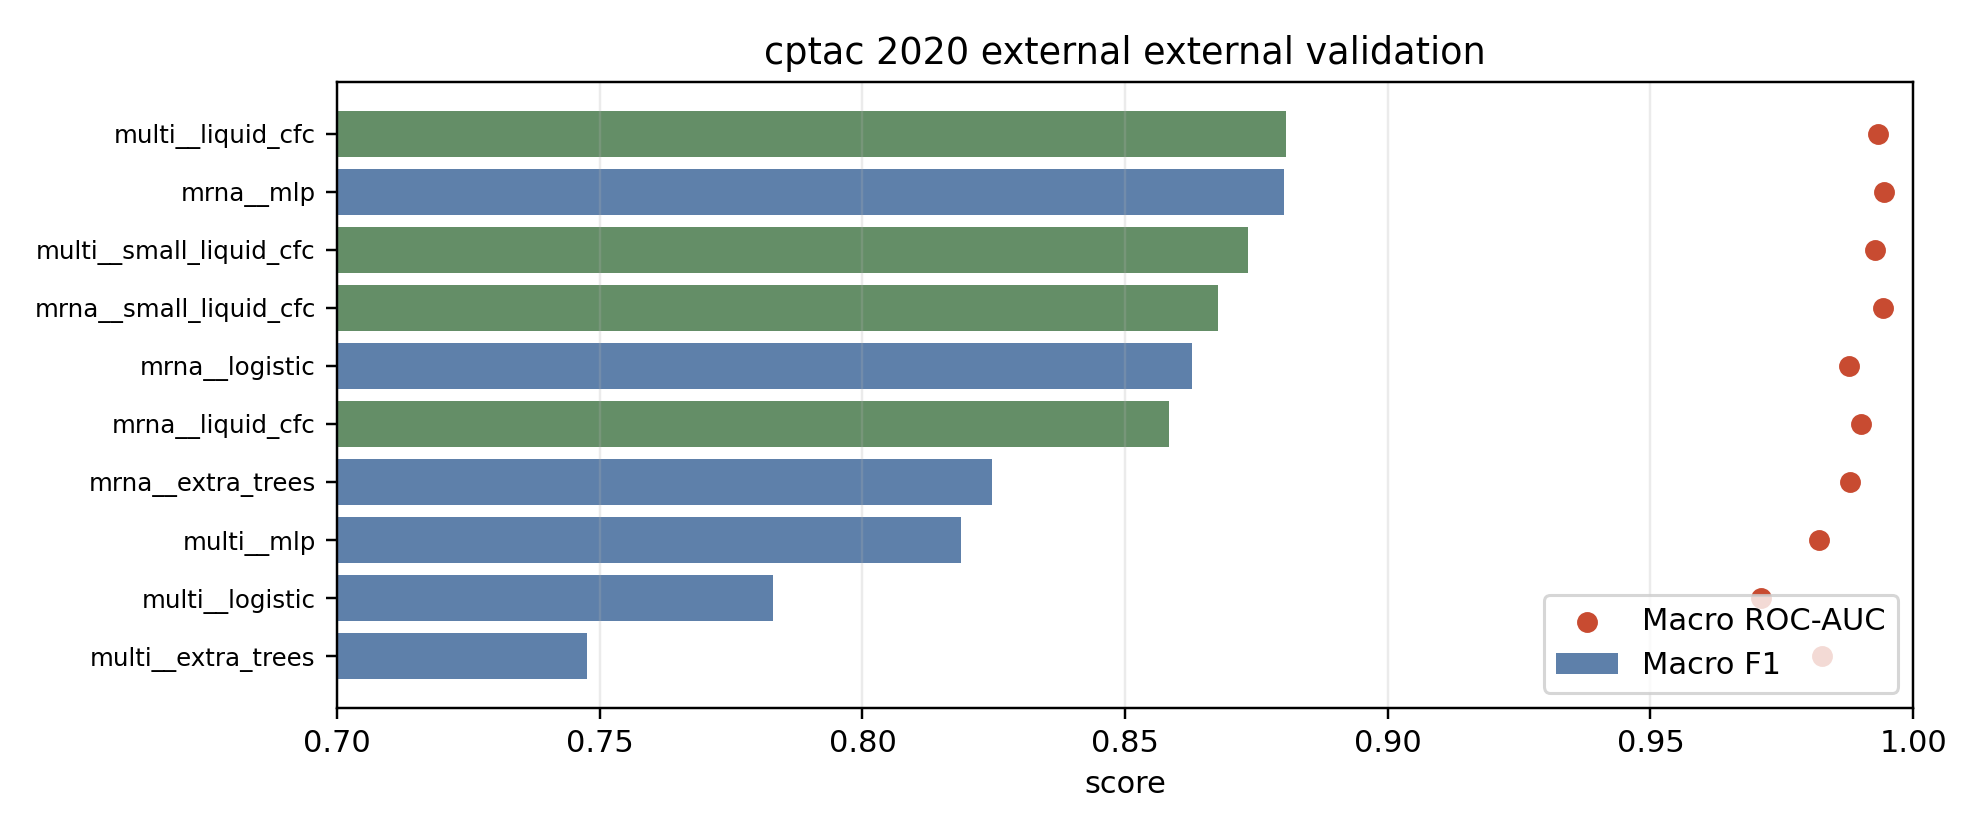
\includegraphics[width=0.85\linewidth]{figures/joined_small_liquid_cptac_2020_external_comparison.png}
\caption{CPTAC 2020 external validation after joined TCGA+METABRIC training.}
\label{fig:cptac}
\end{figure}

\subsection{mRNA-only external validation}

SMC 2018 and SCAN-B were used as mRNA marker external validation cohorts. These cohorts tested cross-cohort transfer of expression-marker models but could not directly evaluate complete multimodal fusion. In SCAN-B, the largest external cohort, ExtraTrees achieved the highest macro F1 (0.8493), followed by Liquid/CfC (0.8172). In SMC 2018, ExtraTrees was also the highest-scoring model (macro F1 = 0.9124), while Liquid/CfC was the strongest neural model (macro F1 = 0.8178).

These results show that strong expression-marker baselines remain difficult to beat when only mRNA features are available. They also indicate that Liquid/CfC is not simply superior by model class; its strongest result emerged in the multimodal CPTAC setting rather than in all expression-only transfers.

\begin{table}[ht]
\centering
\caption{mRNA marker external validation on SCAN-B and SMC 2018.}
\begin{tabular}{llrr}
\toprule
External cohort & Model & Macro F1 & Macro ROC-AUC \\
\midrule
SCAN-B & ExtraTrees & 0.8493 & 0.9831 \\
SCAN-B & Liquid/CfC & 0.8172 & 0.9830 \\
SCAN-B & MLP & 0.8033 & 0.9847 \\
SCAN-B & small-Liquid/CfC & 0.7857 & 0.9818 \\
SCAN-B & Logistic regression & 0.7851 & 0.9801 \\
\midrule
SMC 2018 & ExtraTrees & 0.9124 & 0.9894 \\
SMC 2018 & Liquid/CfC & 0.8178 & 0.9854 \\
SMC 2018 & small-Liquid/CfC & 0.7948 & 0.9838 \\
SMC 2018 & MLP & 0.7799 & 0.9840 \\
SMC 2018 & Logistic regression & 0.7751 & 0.9858 \\
\bottomrule
\end{tabular}
\label{tab:mrna_external}
\end{table}

\begin{figure}[ht]
\centering
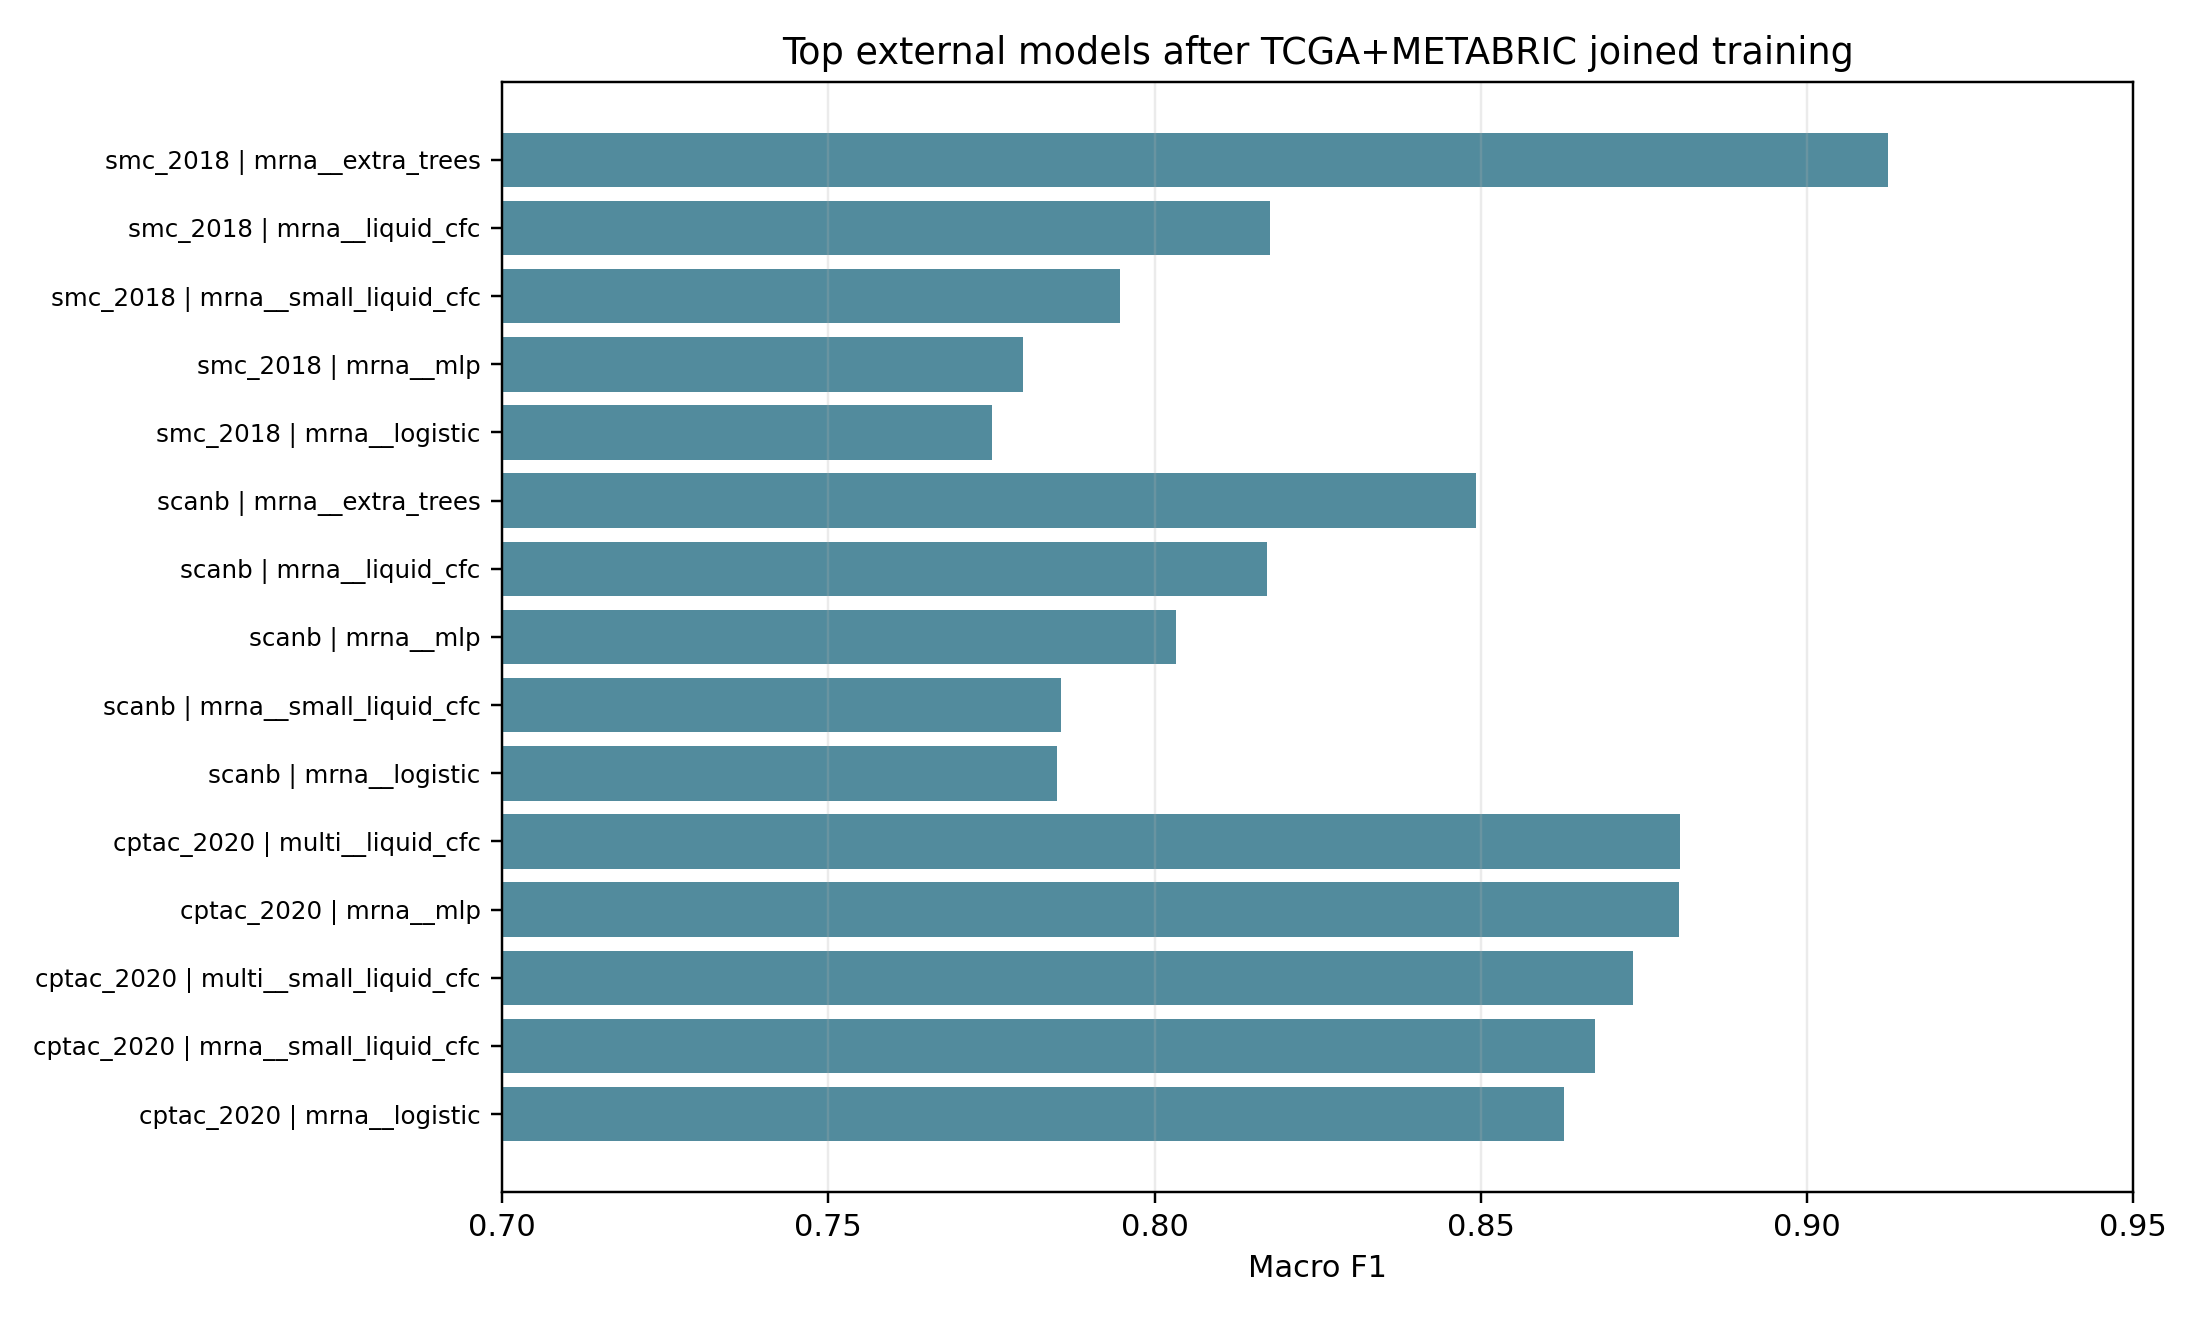
\includegraphics[width=0.9\linewidth]{figures/joined_small_liquid_top_external_macro_f1.png}
\caption{Top external models across CPTAC 2020, SMC 2018, and SCAN-B.}
\label{fig:top_external}
\end{figure}

\subsection{Effect of model-size reduction}

The small-Liquid/CfC model reduced the number of trainable parameters by approximately 68--72\% relative to the original Liquid/CfC model. Despite this reduction, small-Liquid/CfC did not consistently outperform the original model. On CPTAC 2020 multimodal validation, small-Liquid/CfC reached macro F1 of 0.8733, close to but below the original Liquid/CfC score of 0.8806. On SCAN-B and SMC 2018, small-Liquid/CfC was also below the original Liquid/CfC.

Therefore, reducing capacity alone did not solve cross-cohort generalization. The original Liquid/CfC model appeared to have enough capacity to benefit from the enlarged TCGA+METABRIC training pool, whereas the smaller model traded off parameter efficiency for slightly weaker external performance.

\subsection{Extended baseline study and expanded mRNA training scale}

We next expanded the baseline study to include elastic-net logistic regression, calibrated linear SVM, ridge classifier, shrinkage LDA, Gaussian Naive Bayes, k-nearest neighbors, random forest, ExtraTrees, histogram gradient boosting, and an sklearn MLP. This analysis was performed in the mRNA marker setting because SCAN-B and SMC 2018 did not provide the complete CNA and mutation feature set required for clean multimodal training.

Two training scales were compared. The first used the joined TCGA+METABRIC training pool. The second further added SCAN-B and SMC 2018 to create an expanded mRNA training pool, while keeping CPTAC 2020 as the independent external validation cohort. Contrary to a simple sample-size expectation, the expanded mRNA training pool did not improve the best CPTAC external macro F1. Elastic-net logistic regression and sklearn MLP trained on TCGA+METABRIC slightly exceeded multimodal Liquid/CfC on CPTAC macro F1, although the differences were small.

\begin{table}[ht]
\centering
\caption{CPTAC external comparison after extended baseline analysis.}
\resizebox{\textwidth}{!}{%
\begin{tabular}{lllrr}
\toprule
Training scale & Model & Feature set & Macro F1 & Macro ROC-AUC \\
\midrule
TCGA+METABRIC & Logistic ElasticNet & mRNA marker & 0.8830 & 0.9899 \\
TCGA+METABRIC & sklearn MLP & mRNA marker & 0.8823 & 0.9940 \\
TCGA+METABRIC & Liquid/CfC & multimodal marker & 0.8806 & 0.9933 \\
TCGA+METABRIC & MLP & mRNA marker & 0.8803 & 0.9945 \\
TCGA+METABRIC & small-Liquid/CfC & multimodal marker & 0.8733 & 0.9927 \\
Expanded mRNA & sklearn MLP & mRNA marker & 0.8559 & 0.9940 \\
Expanded mRNA & Logistic ElasticNet & mRNA marker & 0.8509 & 0.9911 \\
Expanded mRNA & HistGradientBoosting & mRNA marker & 0.8443 & 0.9869 \\
\bottomrule
\end{tabular}
}
\label{tab:extended_baselines}
\end{table}

\begin{figure}[ht]
\centering
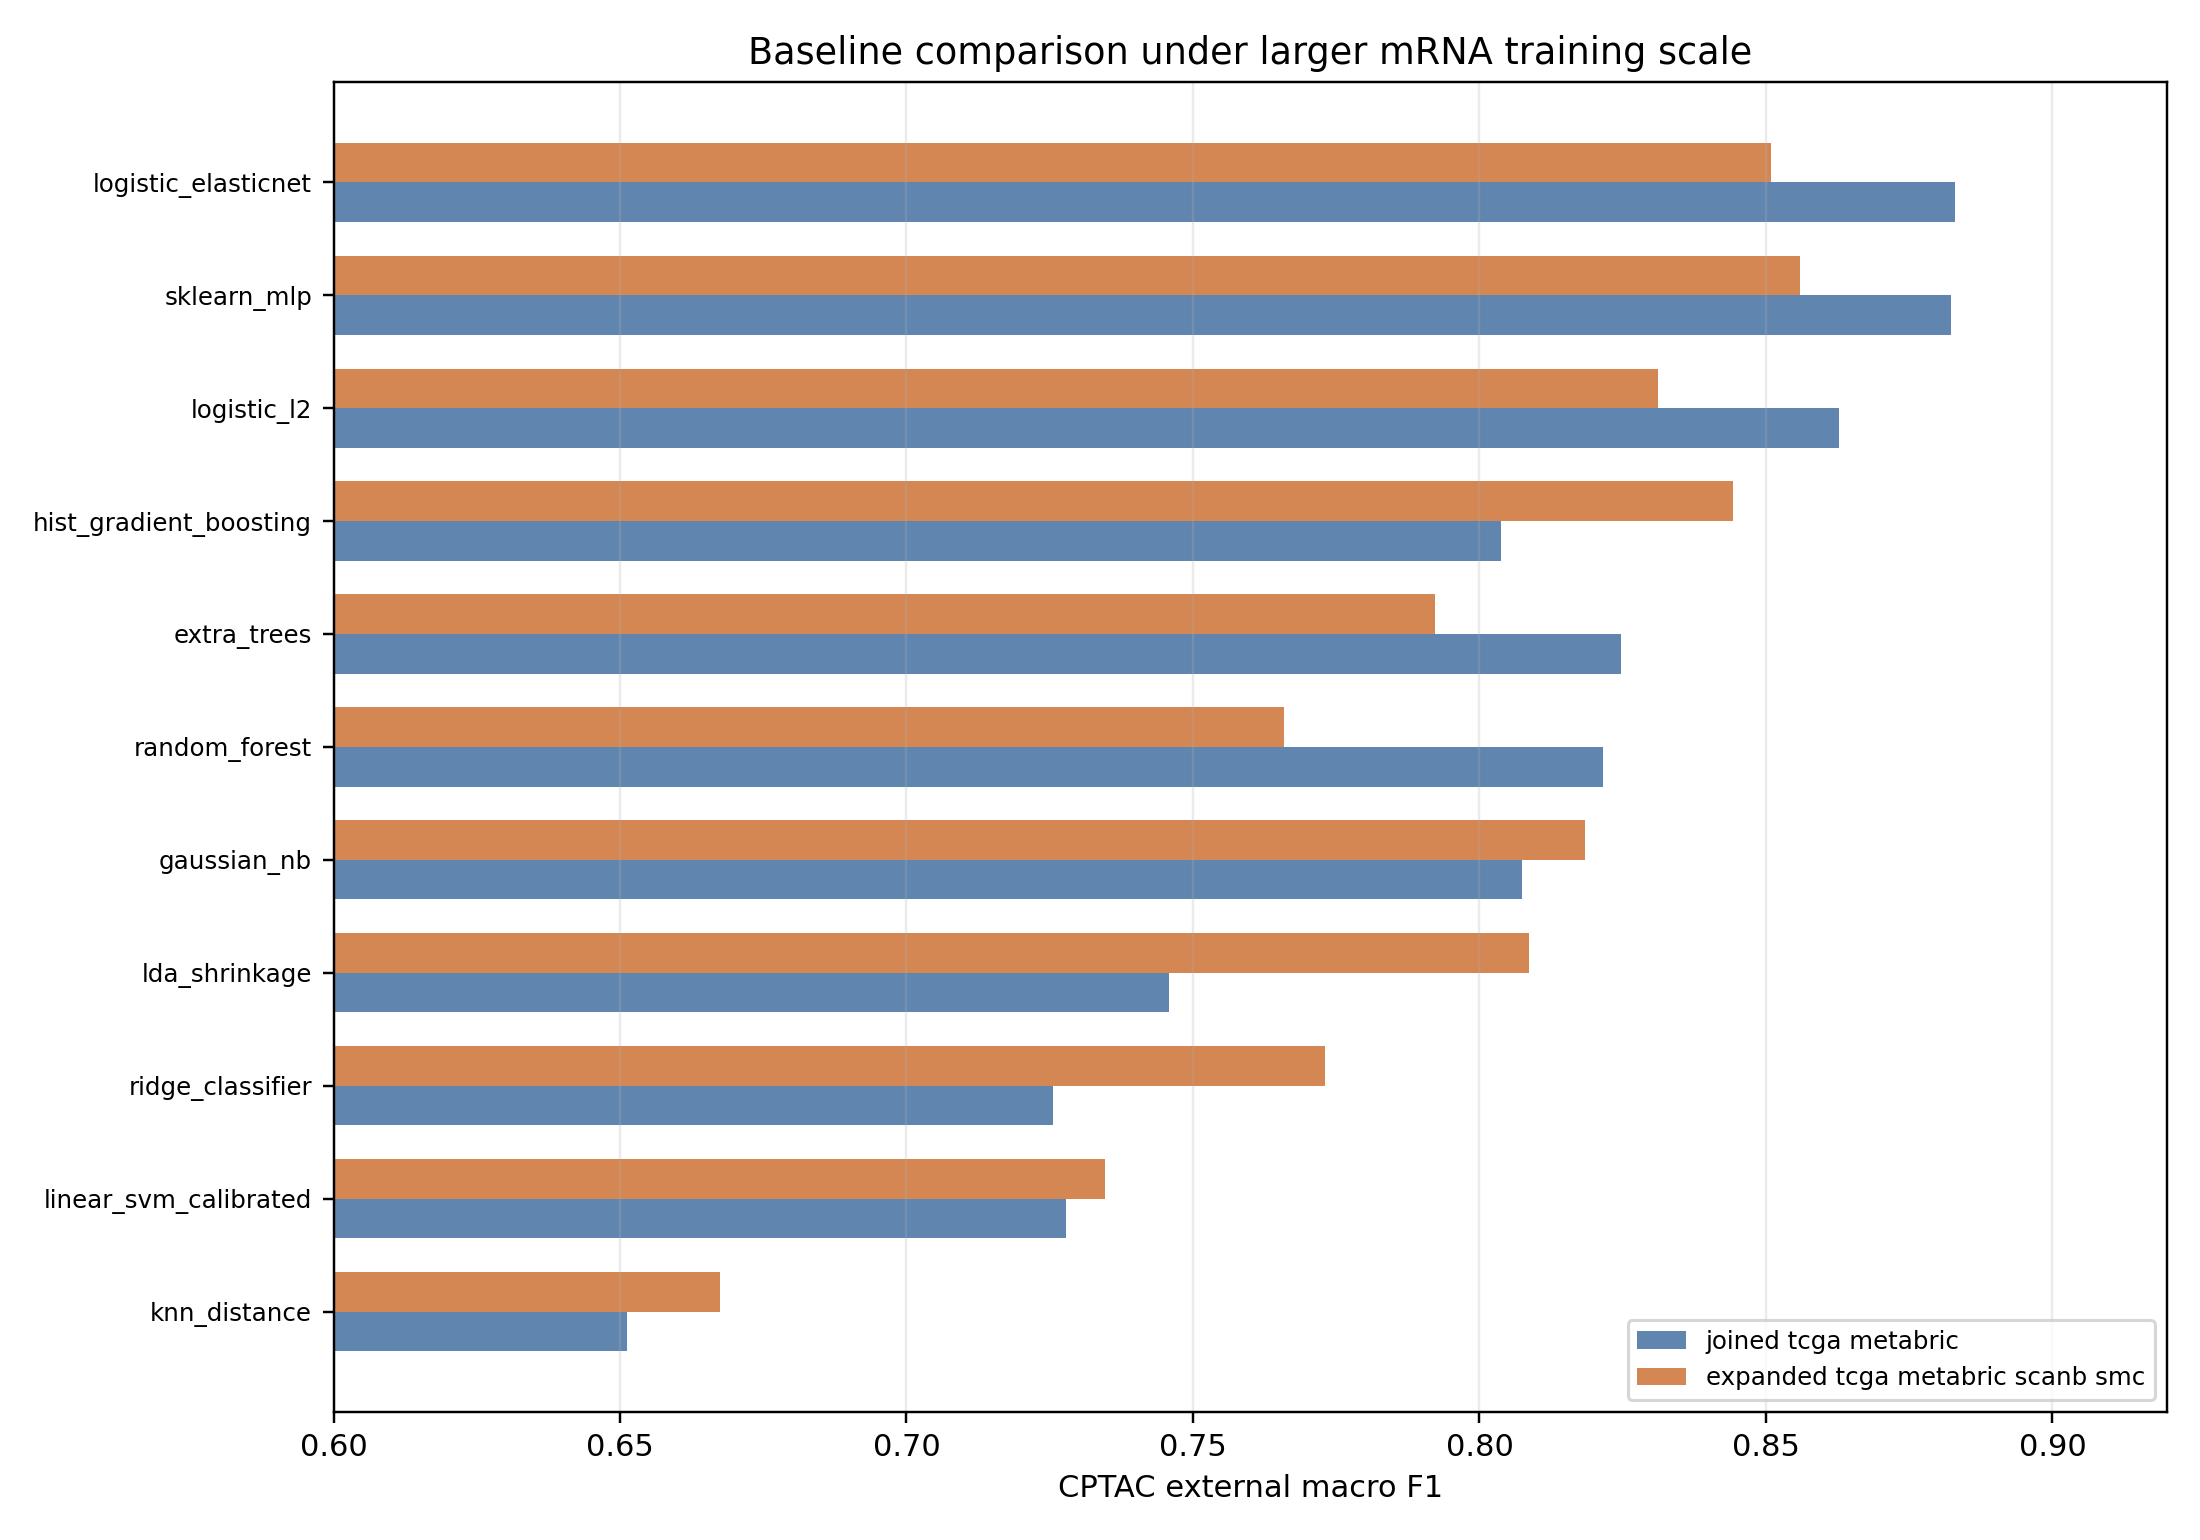
\includegraphics[width=0.9\linewidth]{figures/large_scale_mrna_baseline_cptac_f1.png}
\caption{CPTAC external macro F1 for extended mRNA baselines under TCGA+METABRIC training and expanded TCGA+METABRIC+SCAN-B+SMC training.}
\label{fig:large_baselines}
\end{figure}

\begin{figure}[ht]
\centering
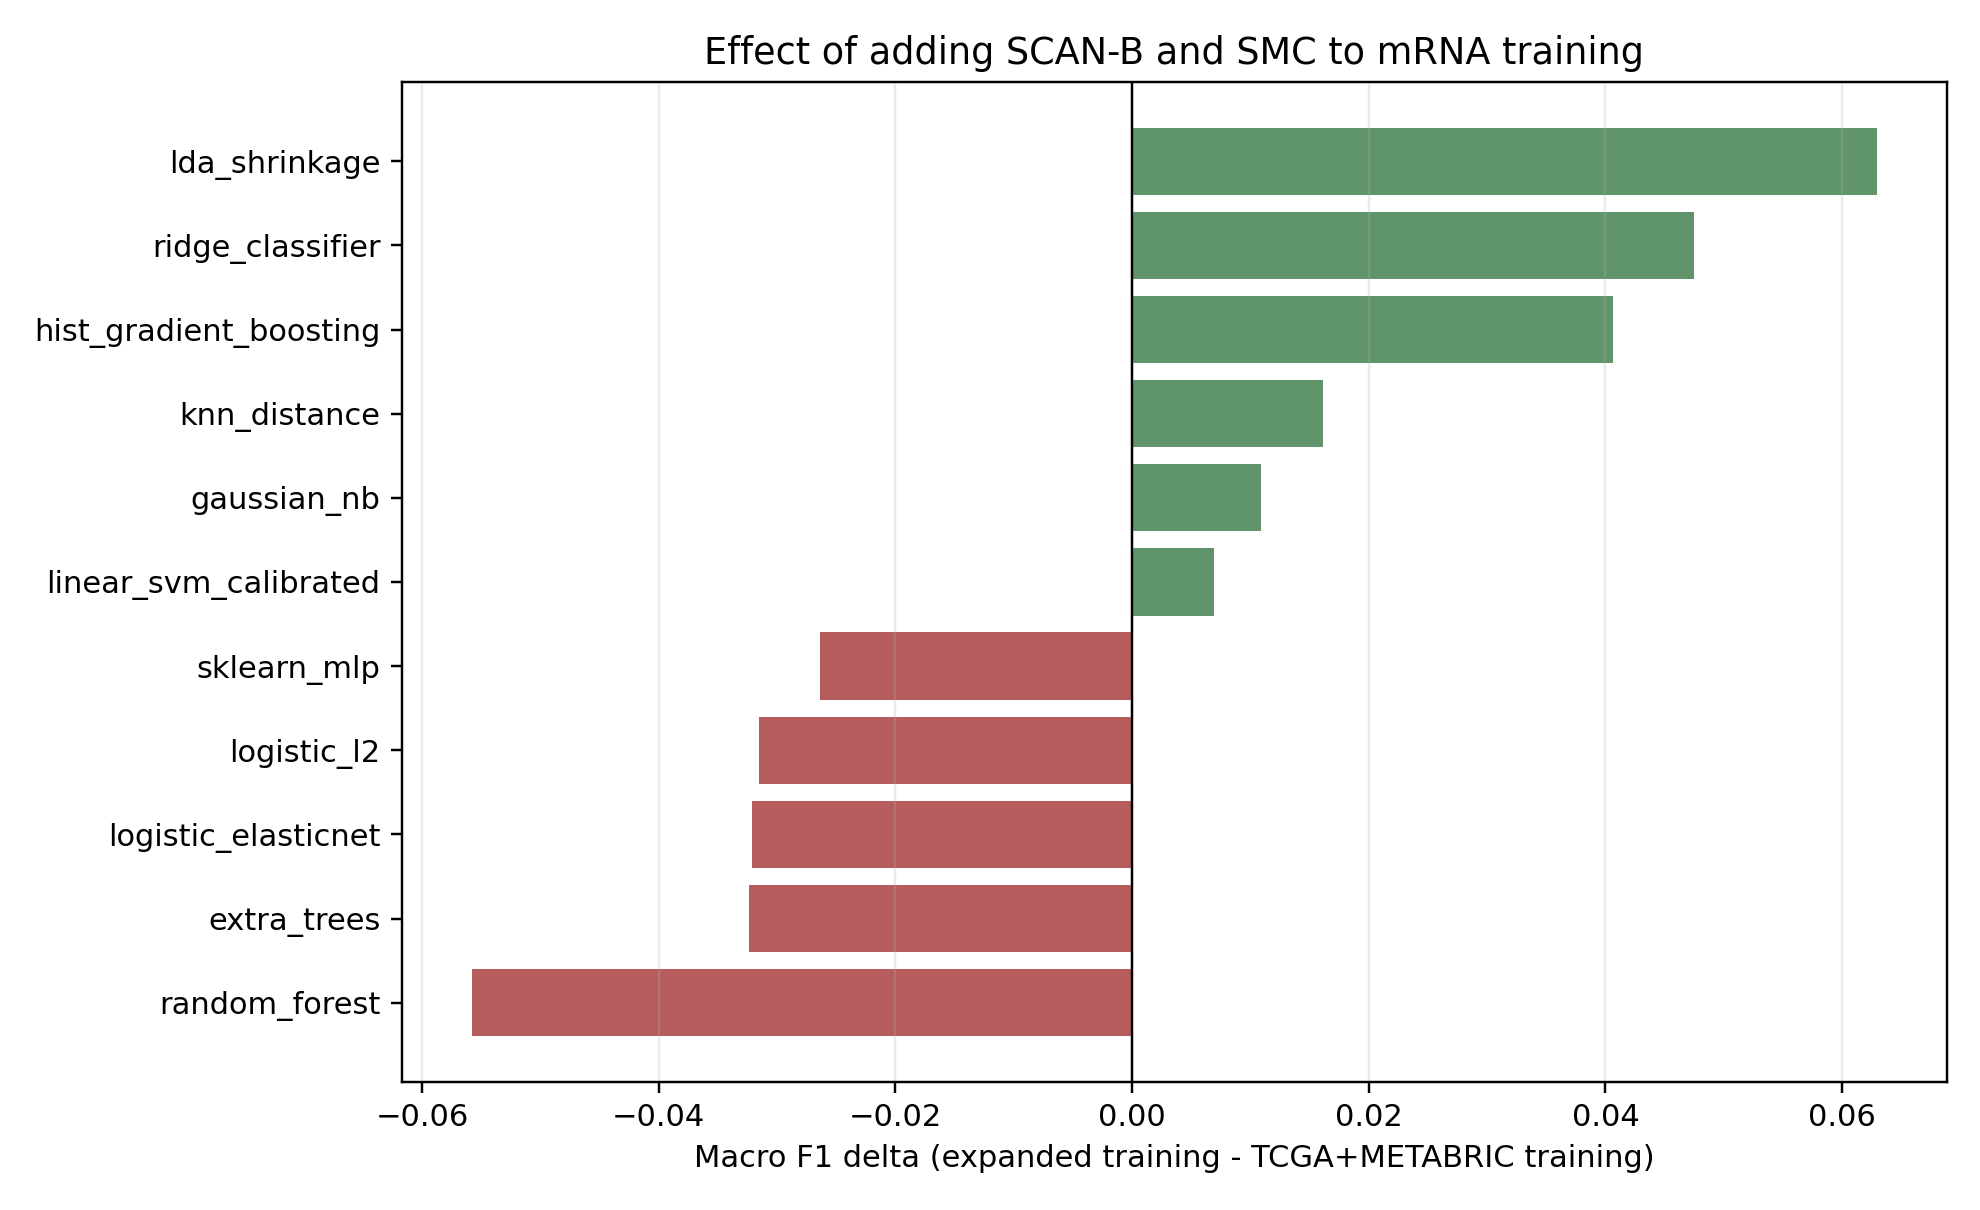
\includegraphics[width=0.85\linewidth]{figures/large_scale_mrna_training_delta_cptac_f1.png}
\caption{Change in CPTAC external macro F1 after adding SCAN-B and SMC 2018 to the mRNA training pool. Negative values indicate reduced external performance after training-scale expansion.}
\label{fig:training_delta}
\end{figure}

\subsection{Multi-cancer internal benchmark}

To move beyond a single-cancer benchmark, we added five cancer-internal prediction tasks from TCGA PanCancer Atlas cohorts. The tasks differed in difficulty. UCEC molecular subtype, COADREAD molecular subtype, and HNSC HPV status were highly predictable, whereas KIRC grade and PRAD pathologic T stage were substantially harder.

No model was best across all tasks. ExtraTrees was strongest for COADREAD molecular subtype and HNSC HPV status. Elastic-net logistic regression was strongest for UCEC molecular subtype. Histogram gradient boosting achieved the highest macro F1 for KIRC grade. small-Liquid/CfC achieved the highest macro F1 for PRAD pathologic T-stage prediction. Complete task-specific model results and label distributions are provided in Supplementary Tables~\ref{tab:supp_label_counts}--\ref{tab:supp_prad}. A core-aligned sensitivity analysis excluding sparse RPPA features is reported in Supplementary Table~\ref{tab:supp_core_aligned}; in that setting, Liquid/CfC was best for COADREAD molecular subtype, whereas other tasks were still led by linear, tree, or boosting baselines. This task-dependent ranking supports the interpretation that Liquid/CfC is a context-dependent fusion candidate rather than a universal winner.

\begin{table}[ht]
\centering
\caption{Best model for each cancer-internal benchmark task.}
\begin{tabular}{llrr}
\toprule
Task & Best model & Macro F1 & Macro ROC-AUC \\
\midrule
HNSC HPV status & ExtraTrees & 0.9505 & 0.9942 \\
UCEC molecular subtype & Logistic ElasticNet & 0.9134 & 0.9831 \\
COADREAD molecular subtype & ExtraTrees & 0.9060 & 0.9546 \\
PRAD pathologic T stage & small-Liquid/CfC & 0.7071 & 0.7717 \\
KIRC grade & HistGradientBoosting & 0.6996 & 0.7556 \\
\bottomrule
\end{tabular}
\label{tab:multicancer_best}
\end{table}

\begin{figure}[ht]
\centering
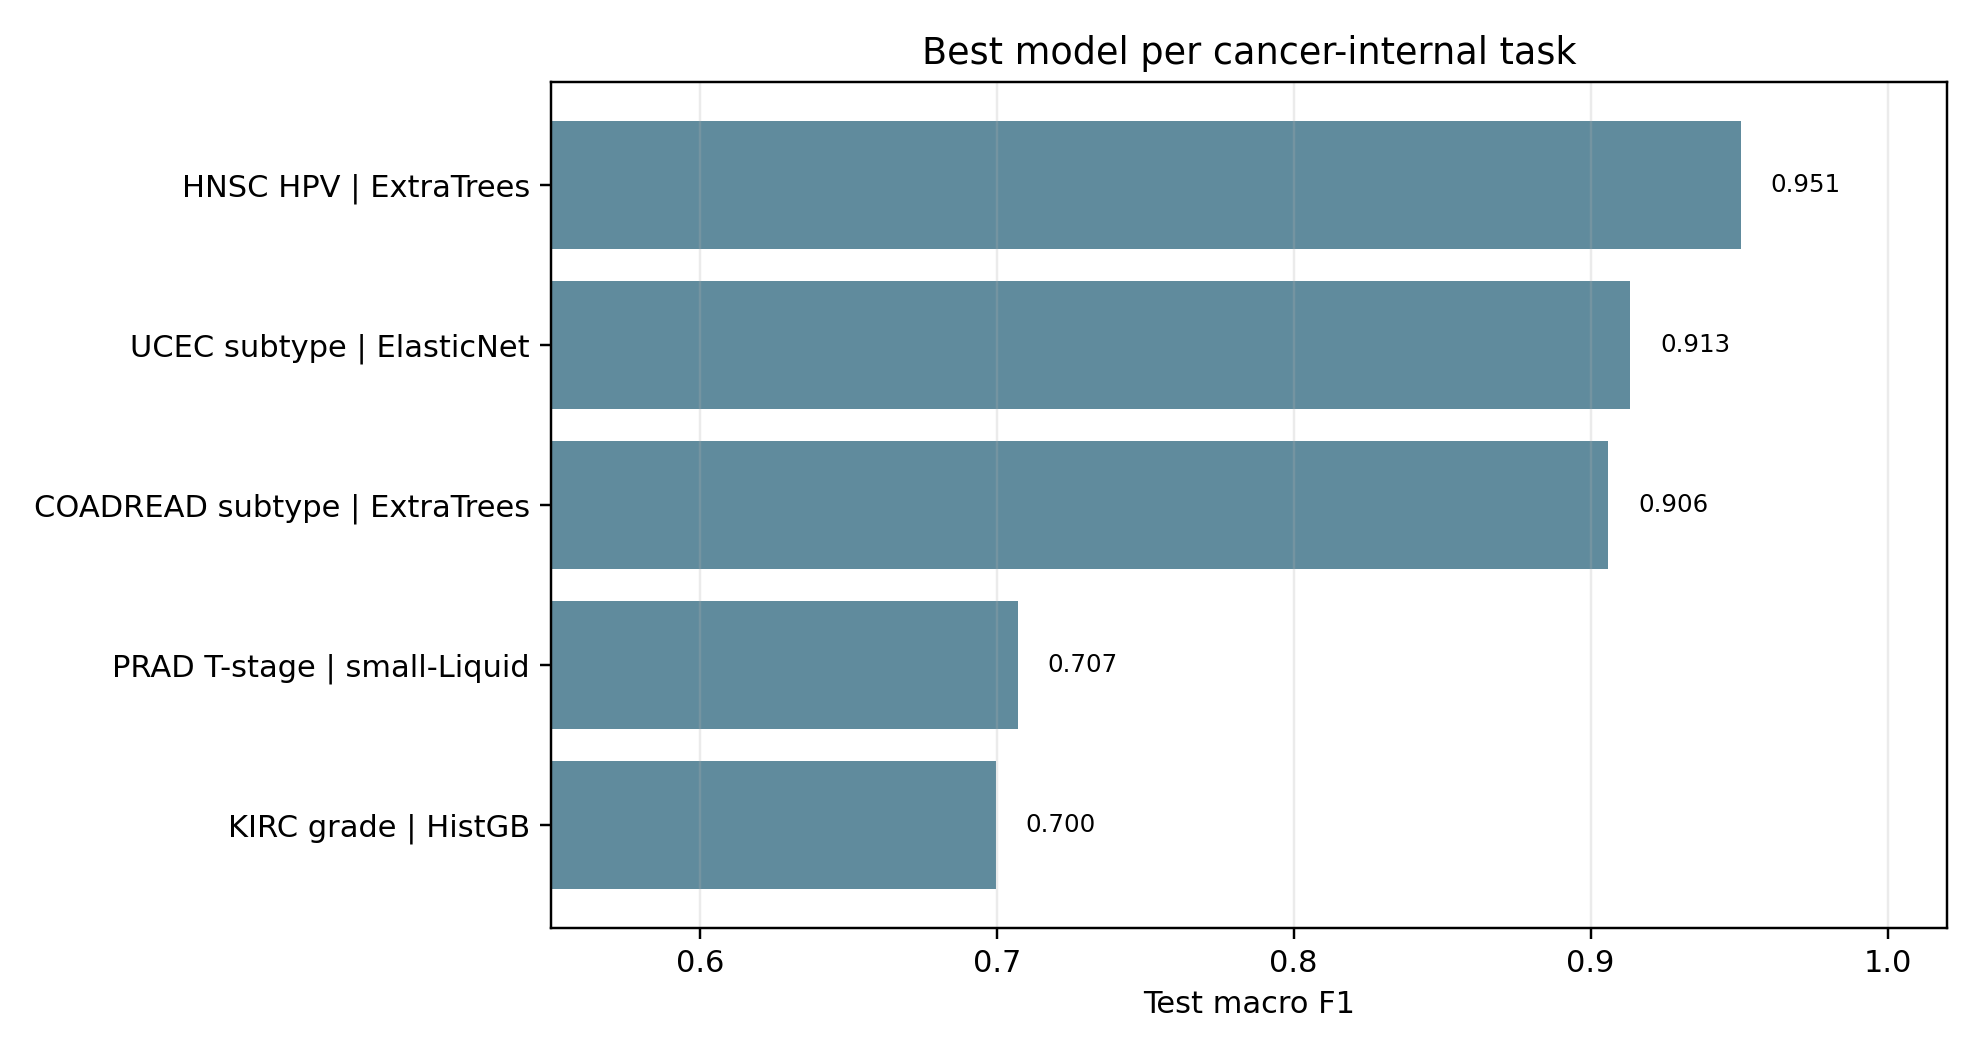
\includegraphics[width=0.85\linewidth]{figures/multicancer_internal_best_by_task.png}
\caption{Best model per cancer-internal benchmark task.}
\label{fig:multicancer_best}
\end{figure}

\begin{figure}[ht]
\centering
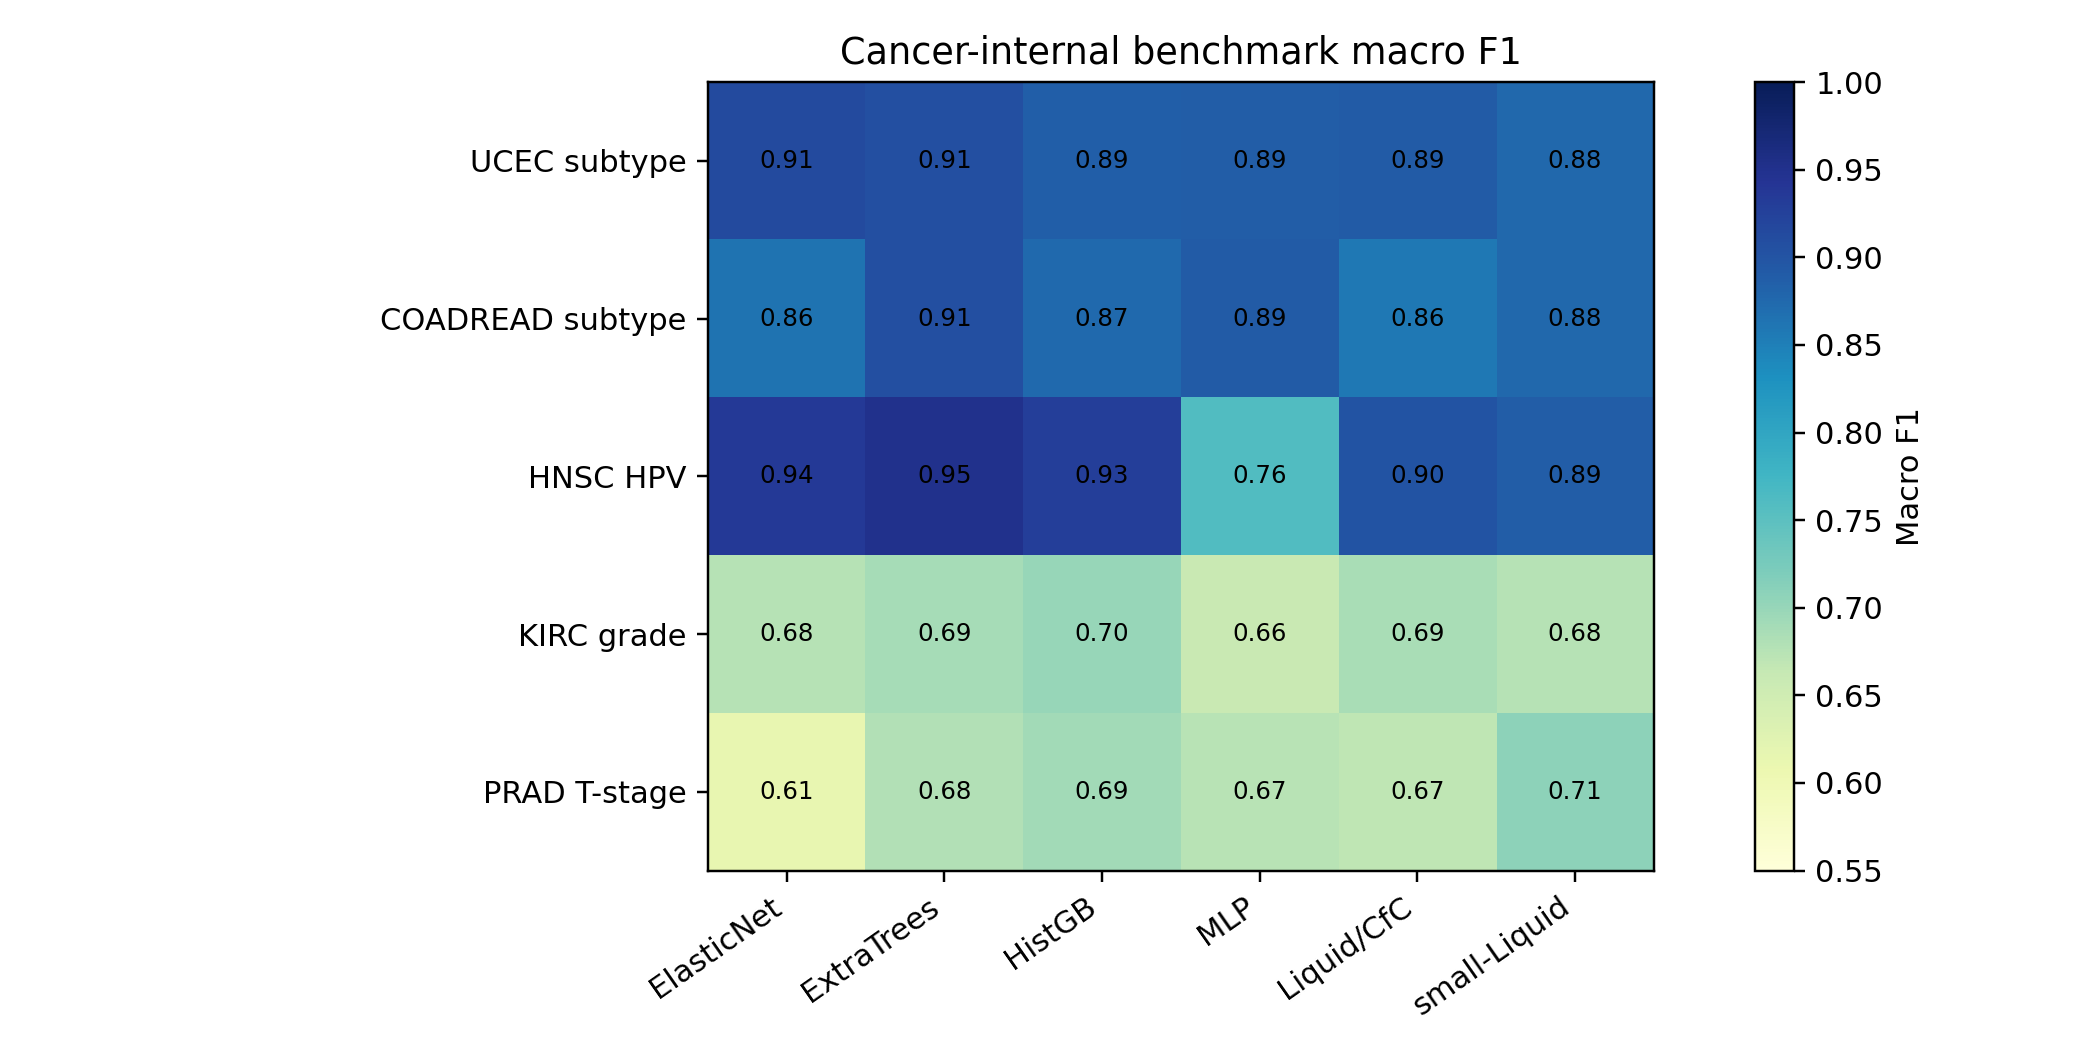
\includegraphics[width=0.95\linewidth]{figures/multicancer_internal_model_task_heatmap.png}
\caption{Macro F1 across models and cancer-internal tasks. The heatmap shows that model ranking is strongly task-dependent.}
\label{fig:multicancer_heatmap}
\end{figure}

\subsection{Cross-validation, significance, and noise robustness}

The ten-fold core-aligned cross-validation analysis confirmed that model ranking varied by task. ExtraTrees was highest for COADREAD molecular subtype (macro F1 = 0.8676), KIRC grade (0.6662), and UCEC molecular subtype (0.8944); logistic ElasticNet was highest for HNSC HPV status (0.9469); and histogram gradient boosting was highest for PRAD pathologic T stage (0.6818). However, none of the top-versus-runner-up paired fold-level comparisons was statistically significant. The paired macro F1 differences were small, ranging from 0.0036 to 0.0159, all bootstrap confidence intervals crossed zero, and the minimum unadjusted paired-test \(p\)-value was 0.375 (Supplementary Table~\ref{tab:supp_cv_significance}). No comparison survived Holm correction across the five tasks. We therefore interpret the task-level rankings as descriptive rather than as evidence of statistically significant universal superiority.

Noise robustness analysis also supported a cautious interpretation. For the best cross-validated model in each task, performance under moderate test-time Gaussian noise was generally stable for HNSC and UCEC but degraded more clearly for COADREAD, KIRC, and PRAD. The estimated noise elbows occurred around \(\sigma=0.30\) for COADREAD, HNSC, KIRC, and UCEC, and around \(\sigma=0.10\) for PRAD (Supplementary Table~\ref{tab:supp_noise_elbow}). PRAD reached a 5\% macro F1 drop by \(\sigma=0.10\), KIRC by \(\sigma=0.20\), and COADREAD by \(\sigma=0.30\), whereas HNSC and UCEC did not reach a 5\% drop by \(\sigma=0.50\). This suggests that some apparent score differences may indeed be within the scale of fold-to-fold and perturbation-level variability.

\subsection{Summary of empirical findings}

The final empirical pattern was cohort- and task-dependent. When aligned multimodal external data were available, as in CPTAC 2020, multimodal Liquid/CfC was highly competitive. However, after strengthening the baseline suite, elastic-net logistic regression and MLP slightly exceeded Liquid/CfC on CPTAC macro F1. On larger mRNA-only external cohorts, expression-marker models and tree-based baselines remained very strong. In the multi-cancer internal benchmark, different model families were optimal for different endpoints. Ten-fold CV and noise analysis further showed that many top-rank differences were small and not statistically significant. Therefore, the evidence supports Liquid/CfC as a useful cross-omics fusion candidate, rather than a universally dominant cancer multi-omics classifier.

\section{Discussion}

This study provides a system-level evaluation of Liquid/CfC-style neural networks for cancer multi-omics prediction. The analysis combines a deep BRCA external-validation study with a broader five-task cancer-internal benchmark. The main conclusion is nuanced. Liquid/CfC did not universally dominate all baselines, especially after the baseline suite was expanded. After increasing the BRCA training data by adding METABRIC, the multimodal Liquid/CfC model was highly competitive on CPTAC 2020, but elastic-net logistic regression and MLP mRNA-marker baselines slightly exceeded it in macro F1.

The results highlight five points. First, breast cancer molecular subtype prediction is strongly driven by subtype-specific expression programs. This explains why mRNA marker models remained highly competitive across external cohorts. Second, multi-omics fusion is not automatically superior to expression-only modeling. It appears most useful when the external cohort has genuinely aligned multi-omics modalities, but even then it must be compared with strong expression baselines. Third, reducing Liquid/CfC capacity through small-Liquid/CfC lowered the parameter count substantially but did not reliably improve external generalization. Fourth, increasing mRNA training scale by adding SCAN-B and SMC 2018 did not improve the best CPTAC external performance, suggesting that cohort and platform shifts can outweigh the benefit of larger sample size. Fifth, the multi-cancer benchmark showed that endpoint difficulty and biological context strongly influence which model family performs best.

These findings argue against overstating Liquid/CfC as a universally superior classifier. A more defensible interpretation is that Liquid/CfC provides an input-adaptive cross-omics state-update mechanism. It is especially relevant when the scientific question concerns how different molecular layers update a latent disease-state representation, rather than simply maximizing subtype classification accuracy.

From a methodological perspective, the study also illustrates why external validation, extensive baseline testing, sample-alignment auditing, cross-validation, and task diversity matter for multi-omics neural networks. A model that appears promising under one internal split may not retain the same ranking across cohorts with different platforms, class distributions, and available modalities. Likewise, a model that is competitive for one endpoint may not be optimal for another. The core-aligned sensitivity analysis showed that removing sparse RPPA features did not turn Liquid/CfC into a universal winner, although it improved the Liquid/CfC ranking for COADREAD molecular subtype in the three-seed split analysis. Ten-fold CV further showed that the top model and runner-up were not significantly different after multiple-testing correction in any internal task. The strongest claim supported by the present results is not that Liquid/CfC replaces simpler baselines, but that it is a competitive and interpretable candidate for cross-omics state-update fusion in selected settings.

\subsection{Limitations}

Several limitations remain. CPTAC 2020 provided multimodal external validation but had only 122 labeled samples, so the strong multimodal Liquid/CfC result should be interpreted cautiously. SMC 2018 and SCAN-B provided independent expression validation but could not test complete mRNA+CNA+mutation fusion. The modality sequence used by Liquid/CfC is biologically motivated but not a true temporal sequence. The TCGA cancer-internal benchmark is sample-ID aligned, but the RPPA block is sparse; therefore, the full RPPA-containing benchmark should be interpreted together with the core-aligned sensitivity analysis. The ten-fold CV and noise analyses suggest that several model differences are small enough to be consistent with random fold-to-fold or perturbation-level variation. Finally, subtype labels can differ across studies due to platform, preprocessing, and annotation differences.

Another limitation is that the final BRCA marker panel was intentionally subtype-focused. This improves biological relevance for breast cancer molecular subtype prediction but limits conclusions about generic cancer-driver panels. The multi-cancer extension partly addresses this limitation, but it remains an internal-split benchmark rather than a multi-cohort external validation for each cancer type. Future studies should add external validation cohorts for UCEC, COADREAD, HNSC, KIRC, and PRAD, and should evaluate endpoints where genomic, epigenomic, proteomic, and transcriptomic layers provide complementary information, such as treatment response, recurrence risk, or survival.

\subsection{Conclusion}

Adding METABRIC to the training pool improved the viability of Liquid/CfC for external breast cancer subtype prediction. The original Liquid/CfC model outperformed the reduced small-Liquid model in most BRCA external settings and was highly competitive on CPTAC 2020 multimodal validation. Nevertheless, strengthened expression-marker baselines slightly exceeded Liquid/CfC on CPTAC macro F1, and larger mRNA training scale did not improve the best external performance. In the multi-cancer internal benchmark, the best model varied by endpoint, and ten-fold CV did not show statistically significant top-versus-runner-up differences after correction. The most appropriate conclusion is that Liquid/CfC is a promising but context-dependent cross-omics fusion architecture, not a universally dominant model.

\section*{Declarations}

\subsection*{Funding}

No specific funding was received for this work.

\subsection*{Conflicts of interest/Competing interests}

The authors declare that they have no competing interests.

\subsection*{Ethics approval and consent to participate}

Not applicable. This study used publicly available, de-identified molecular and clinical datasets.

\subsection*{Availability of data and material}

All datasets used in this study are publicly available. TCGA-BRCA, TCGA PanCancer Atlas cohorts, METABRIC, CPTAC 2020, and SMC 2018 molecular and clinical data were accessed through cBioPortal. GSE96058/SCAN-B data were accessed through the Gene Expression Omnibus and the associated public processed data package. Analysis scripts, compact processed result tables, figures, reports, and the manuscript source are available in the public GitHub repository: \url{https://github.com/123hzq321/cancer-multiomics-learning-models-benchmark}.

\subsection*{Code availability}

Analysis scripts used to download, preprocess, train, and evaluate the models are available at \url{https://github.com/123hzq321/cancer-multiomics-learning-models-benchmark}. Key scripts include:
\begingroup
\footnotesize
\begin{itemize}
\item \path{train_joined_metabric_small_liquid_external_validation.py}
\item \path{train_large_scale_mrna_baselines.py}
\item \path{train_multicancer_internal_benchmark.py}
\item \path{reviewer_cv_noise_significance_analysis.py}
\end{itemize}
\endgroup

\subsection*{Consent for publication}

Not applicable.

\subsection*{Authors' contributions}

Z.H. conceived the study, designed the computational experiments, processed the data, implemented the analysis pipeline, performed model training and evaluation, prepared figures and tables, and drafted the manuscript. X.B. supervised the study, contributed clinical interpretation, and revised the manuscript. Both authors reviewed and approved the final manuscript.

\subsection*{Acknowledgements}

Not applicable.


\clearpage
\appendix
\section{Supplementary Tables}

\setcounter{table}{0}
\renewcommand{\thetable}{S\arabic{table}}

The supplementary tables report cancer-internal label distributions (Supplementary Table~\ref{tab:supp_label_counts}), task-specific benchmark results for UCEC (Supplementary Table~\ref{tab:supp_ucec}), COADREAD (Supplementary Table~\ref{tab:supp_coadread}), HNSC (Supplementary Table~\ref{tab:supp_hnsc}), KIRC (Supplementary Table~\ref{tab:supp_kirc}), and PRAD (Supplementary Table~\ref{tab:supp_prad}), the sample-alignment audit (Supplementary Table~\ref{tab:supp_alignment}), the core-aligned sensitivity analysis (Supplementary Table~\ref{tab:supp_core_aligned}), ten-fold cross-validation results (Supplementary Table~\ref{tab:supp_cv_best}), fold-level paired comparisons (Supplementary Table~\ref{tab:supp_cv_significance}), and noise robustness results (Supplementary Table~\ref{tab:supp_noise_elbow}).

\begin{table}[ht]
\centering
\caption{Cancer-internal task label distributions.}
\begin{tabular}{llr}
\toprule
Task & Label & Samples \\
\midrule
UCEC molecular subtype & CN\_HIGH & 163 \\
UCEC molecular subtype & MSI & 148 \\
UCEC molecular subtype & CN\_LOW & 147 \\
UCEC molecular subtype & POLE & 49 \\
COADREAD molecular subtype & CIN & 328 \\
COADREAD molecular subtype & MSI & 63 \\
COADREAD molecular subtype & GS & 58 \\
HNSC HPV status & HPV\_NEG & 415 \\
HNSC HPV status & HPV\_POS & 72 \\
KIRC grade & HIGH\_GRADE & 277 \\
KIRC grade & LOW\_GRADE & 227 \\
PRAD pathologic T stage & T3\_T4 & 300 \\
PRAD pathologic T stage & T2 & 187 \\
\bottomrule
\end{tabular}
\label{tab:supp_label_counts}
\end{table}

\begin{table}[ht]
\centering
\caption{UCEC molecular subtype benchmark results. Values are mean $\pm$ standard deviation across three random seeds.}
\begin{tabular}{lrr}
\toprule
Model & Macro F1 & Macro ROC-AUC \\
\midrule
Logistic ElasticNet & 0.913 $\pm$ 0.050 & 0.983 $\pm$ 0.010 \\
ExtraTrees & 0.906 $\pm$ 0.053 & 0.984 $\pm$ 0.008 \\
Liquid/CfC & 0.890 $\pm$ 0.051 & 0.986 $\pm$ 0.007 \\
MLP & 0.888 $\pm$ 0.027 & 0.978 $\pm$ 0.012 \\
HistGradientBoosting & 0.887 $\pm$ 0.055 & 0.983 $\pm$ 0.006 \\
small-Liquid/CfC & 0.876 $\pm$ 0.077 & 0.985 $\pm$ 0.014 \\
\bottomrule
\end{tabular}
\label{tab:supp_ucec}
\end{table}

\begin{table}[ht]
\centering
\caption{COADREAD molecular subtype benchmark results. Values are mean $\pm$ standard deviation across three random seeds.}
\begin{tabular}{lrr}
\toprule
Model & Macro F1 & Macro ROC-AUC \\
\midrule
ExtraTrees & 0.906 $\pm$ 0.049 & 0.955 $\pm$ 0.007 \\
MLP & 0.891 $\pm$ 0.043 & 0.973 $\pm$ 0.008 \\
small-Liquid/CfC & 0.876 $\pm$ 0.030 & 0.956 $\pm$ 0.021 \\
HistGradientBoosting & 0.875 $\pm$ 0.034 & 0.959 $\pm$ 0.010 \\
Logistic ElasticNet & 0.863 $\pm$ 0.019 & 0.968 $\pm$ 0.001 \\
Liquid/CfC & 0.858 $\pm$ 0.025 & 0.969 $\pm$ 0.004 \\
\bottomrule
\end{tabular}
\label{tab:supp_coadread}
\end{table}

\begin{table}[ht]
\centering
\caption{HNSC HPV status benchmark results. Values are mean $\pm$ standard deviation across three random seeds.}
\begin{tabular}{lrr}
\toprule
Model & Macro F1 & Macro ROC-AUC \\
\midrule
ExtraTrees & 0.951 $\pm$ 0.046 & 0.994 $\pm$ 0.010 \\
Logistic ElasticNet & 0.936 $\pm$ 0.045 & 0.977 $\pm$ 0.030 \\
HistGradientBoosting & 0.928 $\pm$ 0.042 & 0.986 $\pm$ 0.016 \\
Liquid/CfC & 0.902 $\pm$ 0.036 & 0.977 $\pm$ 0.032 \\
small-Liquid/CfC & 0.889 $\pm$ 0.126 & 0.964 $\pm$ 0.034 \\
MLP & 0.760 $\pm$ 0.051 & 0.992 $\pm$ 0.013 \\
\bottomrule
\end{tabular}
\label{tab:supp_hnsc}
\end{table}

\begin{table}[ht]
\centering
\caption{KIRC grade benchmark results. Values are mean $\pm$ standard deviation across three random seeds.}
\begin{tabular}{lrr}
\toprule
Model & Macro F1 & Macro ROC-AUC \\
\midrule
HistGradientBoosting & 0.700 $\pm$ 0.016 & 0.756 $\pm$ 0.008 \\
ExtraTrees & 0.688 $\pm$ 0.049 & 0.753 $\pm$ 0.041 \\
Liquid/CfC & 0.686 $\pm$ 0.021 & 0.770 $\pm$ 0.051 \\
Logistic ElasticNet & 0.676 $\pm$ 0.079 & 0.705 $\pm$ 0.046 \\
small-Liquid/CfC & 0.675 $\pm$ 0.059 & 0.718 $\pm$ 0.043 \\
MLP & 0.659 $\pm$ 0.062 & 0.751 $\pm$ 0.041 \\
\bottomrule
\end{tabular}
\label{tab:supp_kirc}
\end{table}

\begin{table}[ht]
\centering
\caption{PRAD pathologic T-stage benchmark results. Values are mean $\pm$ standard deviation across three random seeds.}
\begin{tabular}{lrr}
\toprule
Model & Macro F1 & Macro ROC-AUC \\
\midrule
small-Liquid/CfC & 0.707 $\pm$ 0.065 & 0.772 $\pm$ 0.044 \\
HistGradientBoosting & 0.692 $\pm$ 0.027 & 0.748 $\pm$ 0.065 \\
ExtraTrees & 0.679 $\pm$ 0.016 & 0.780 $\pm$ 0.048 \\
MLP & 0.674 $\pm$ 0.057 & 0.768 $\pm$ 0.023 \\
Liquid/CfC & 0.669 $\pm$ 0.070 & 0.732 $\pm$ 0.093 \\
Logistic ElasticNet & 0.614 $\pm$ 0.048 & 0.704 $\pm$ 0.101 \\
\bottomrule
\end{tabular}
\label{tab:supp_prad}
\end{table}

\begin{table}[ht]
\centering
\caption{Sample-alignment audit. Each labelled analysis table contains one row per sample identifier and no duplicated sample IDs after endpoint filtering.}
\resizebox{\textwidth}{!}{%
\begin{tabular}{llrrrl}
\toprule
Analysis & Dataset & Samples & Unique IDs & Duplicate IDs & Compatible experiment \\
\midrule
BRCA joined training & TCGA+METABRIC & 2737 & 2737 & 0 & mRNA and multimodal \\
BRCA external validation & CPTAC 2020 & 122 & 122 & 0 & mRNA and multimodal \\
BRCA external validation & SMC 2018 & 168 & 168 & 0 & mRNA-only comparison \\
BRCA external validation & SCAN-B/GSE96058 & 3137 & 3137 & 0 & mRNA-only comparison \\
TCGA internal benchmark & UCEC molecular subtype & 507 & 507 & 0 & aligned internal multi-omics \\
TCGA internal benchmark & COADREAD molecular subtype & 449 & 449 & 0 & aligned internal multi-omics \\
TCGA internal benchmark & HNSC HPV status & 487 & 487 & 0 & aligned internal multi-omics \\
TCGA internal benchmark & KIRC grade & 504 & 504 & 0 & aligned internal multi-omics \\
TCGA internal benchmark & PRAD pathologic T stage & 487 & 487 & 0 & aligned internal multi-omics \\
\bottomrule
\end{tabular}
}
\label{tab:supp_alignment}
\end{table}

\begin{table}[ht]
\centering
\caption{Core-aligned cancer-internal sensitivity analysis excluding sparse RPPA features. Values are mean $\pm$ standard deviation across three random seeds.}
\resizebox{\textwidth}{!}{%
\begin{tabular}{llrr}
\toprule
Task & Best model & Macro F1 & Macro ROC-AUC \\
\midrule
COADREAD molecular subtype & Liquid/CfC & 0.918 $\pm$ 0.011 & 0.967 $\pm$ 0.013 \\
HNSC HPV status & Logistic ElasticNet & 0.943 $\pm$ 0.034 & 0.978 $\pm$ 0.030 \\
KIRC grade & ExtraTrees & 0.711 $\pm$ 0.044 & 0.741 $\pm$ 0.055 \\
PRAD pathologic T stage & HistGradientBoosting & 0.703 $\pm$ 0.062 & 0.755 $\pm$ 0.079 \\
UCEC molecular subtype & Logistic ElasticNet & 0.910 $\pm$ 0.045 & 0.982 $\pm$ 0.011 \\
\bottomrule
\end{tabular}
}
\label{tab:supp_core_aligned}
\end{table}

\begin{table}[ht]
\centering
\caption{Ten-fold cross-validation best model per core-aligned cancer-internal task. RPPA was excluded from this sensitivity analysis.}
\resizebox{\textwidth}{!}{%
\begin{tabular}{llrr}
\toprule
Task & Best model & Macro F1 & Macro ROC-AUC \\
\midrule
COADREAD molecular subtype & ExtraTrees & 0.868 $\pm$ 0.069 & 0.955 \\
HNSC HPV status & Logistic ElasticNet & 0.947 $\pm$ 0.038 & 0.961 \\
KIRC grade & ExtraTrees & 0.666 $\pm$ 0.064 & 0.730 \\
PRAD pathologic T stage & HistGradientBoosting & 0.682 $\pm$ 0.039 & 0.749 \\
UCEC molecular subtype & ExtraTrees & 0.894 $\pm$ 0.068 & 0.983 \\
\bottomrule
\end{tabular}
}
\label{tab:supp_cv_best}
\end{table}

\begin{table}[ht]
\centering
\caption{Fold-level top-versus-runner-up comparison in ten-fold cross-validation. Raw paired-test \(p\)-values are shown; no comparison survived Holm correction across the five tasks.}
\resizebox{\textwidth}{!}{%
\begin{tabular}{lllcrrrr}
\toprule
Task & Top model & Runner-up & Top wins & Mean F1 difference & 95\% CI low & 95\% CI high & Raw \(p\) \\
\midrule
COADREAD molecular subtype & ExtraTrees & small-Liquid/CfC & 5/10 & 0.005 & -0.043 & 0.051 & 1.000 \\
HNSC HPV status & Logistic ElasticNet & HistGradientBoosting & 5/10 & 0.016 & -0.014 & 0.047 & 0.375 \\
KIRC grade & ExtraTrees & HistGradientBoosting & 7/10 & 0.013 & -0.038 & 0.061 & 0.557 \\
PRAD pathologic T stage & HistGradientBoosting & ExtraTrees & 5/10 & 0.004 & -0.028 & 0.032 & 0.826 \\
UCEC molecular subtype & ExtraTrees & Logistic ElasticNet & 7/10 & 0.005 & -0.039 & 0.047 & 0.695 \\
\bottomrule
\end{tabular}
}
\label{tab:supp_cv_significance}
\end{table}

\begin{table}[ht]
\centering
\caption{Noise robustness and estimated elbow for the best cross-validated model in each core-aligned task. Noise was added to standardized test features after training.}
\resizebox{\textwidth}{!}{%
\begin{tabular}{llrrrrr}
\toprule
Task & Model & Clean F1 & F1 at \(\sigma=0.20\) & F1 at \(\sigma=0.50\) & First 5\% drop & Elbow \(\sigma\) \\
\midrule
COADREAD molecular subtype & ExtraTrees & 0.868 & 0.847 & 0.736 & 0.30 & 0.30 \\
HNSC HPV status & Logistic ElasticNet & 0.947 & 0.940 & 0.943 & Not reached & 0.30 \\
KIRC grade & ExtraTrees & 0.666 & 0.628 & 0.514 & 0.20 & 0.30 \\
PRAD pathologic T stage & HistGradientBoosting & 0.682 & 0.570 & 0.482 & 0.10 & 0.10 \\
UCEC molecular subtype & ExtraTrees & 0.894 & 0.894 & 0.860 & Not reached & 0.30 \\
\bottomrule
\end{tabular}
}
\label{tab:supp_noise_elbow}
\end{table}

\clearpage

\bibliographystyle{unsrt}
\bibliography{references}

\end{document}
